\documentclass[14Q,twocolumn]{jsarticle}
\usepackage[dvipdfmx]{graphicx}
\usepackage{wrapfig}
\usepackage{float}
\usepackage{otf}
\usepackage{longtable}
\usepackage{ulem}
\usepackage{ascmac}
\usepackage{multicol}
%%%%%
\makeatletter
\newenvironment{tablehere}
  {\def\@captype{table}}
  {}
\newenvironment{figurehere}
  {\def\@captype{figure}}
  {}
\makeatother
%%%%%%
\setlength{\textwidth}{160truemm}      % テキスト幅: 160mm
\setlength{\fullwidth}{\textwidth}     % ページ全体の幅
\setlength{\oddsidemargin}{0mm}   % 左余白
\setlength{\topmargin}{-10mm}       % 上余白
\setlength{\textheight}{240truemm}     % テキスト高さ: 297-(30+30)=237mm
\pagestyle{empty}
\title{QGISで等高線}% 文書のタイトル
\date{2018年9月18日}
\author{厚沢部町 石 井 淳 平}              % 著者

%------------------------------
\begin{document}
\maketitle
%\begin{multicols}{2}
\section{この時間に覚えること}
この演習ではラスタデータ(紙地図)からベクタデータ(ポイントデータ)を作成し、ベクタデータからラスタデータ(標高ラスタ)を生成し、さらにもう一度ベクタデータ(等高線)を生成するという複雑な手順を行います。一連の作業でベクタデータとラスタデータの特徴を理解します。

\begin{itemize}
\item 紙図面から標高値を取得してポイントベクタを作成する。
\item  ポイントベクタから標高ラスタを作成する。
\item  標高ラスタから等高線を発生させる。
\end{itemize}


%%%%
\section{新規にベクタレイヤを作成する}
GISデータの場合、地物のタイプが限定されます。「ポイント」、「ライン」、「ポリゴン」の3種類です。基本的にこれらのデータは異なる性質をもつため別々のデータとして格納されます。ポイントデータとラインデータが混在することはできません。

\begin{tabular}{l l}
タイプ&点\\
ファイルエンコーディング&UTF-8\\
CRSの指定&後ほど説明\\
名称&Level\\
タイプ&小数点付き数値\\
EPSGコード&30171\\
\end{tabular}

\begin{figurehere}
\centering
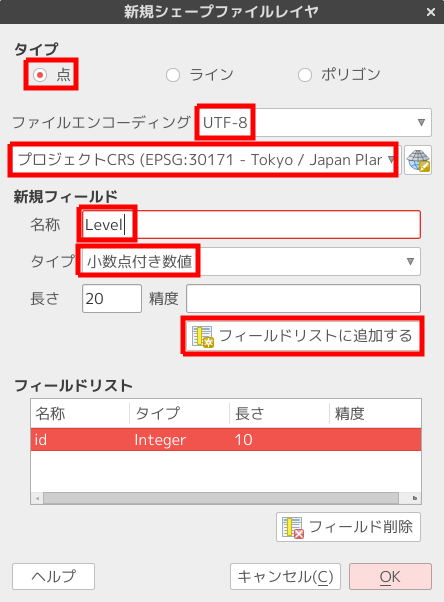
\includegraphics[width=0.5\linewidth]{02.png}
\caption{新しいシェープファイルの作成}
\end{figurehere}

\begin{figurehere}
\centering
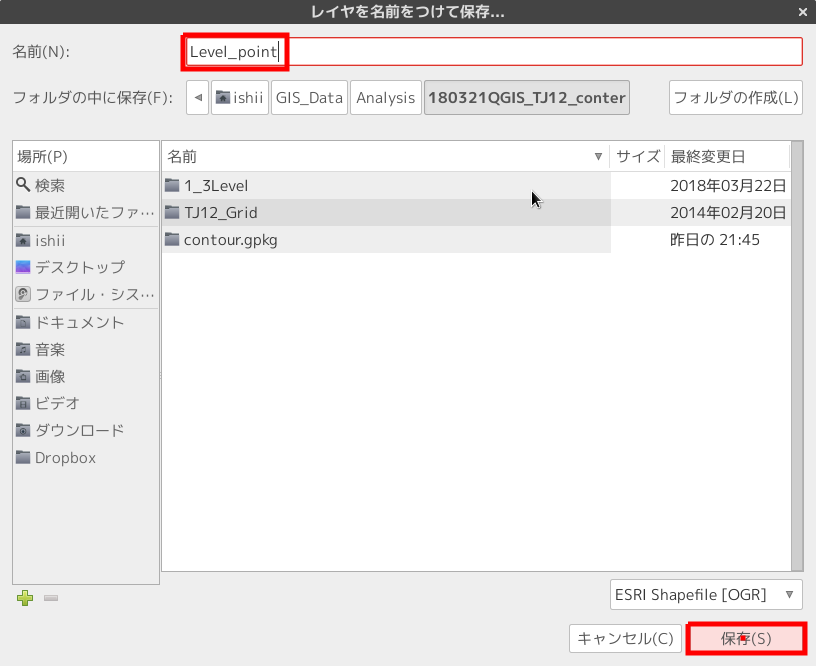
\includegraphics[width=0.8\linewidth]{03.png}
\caption{空間参照系(測地系・座標系)を選択}
\end{figurehere}

%%%%
\section{紙図面から標高データを取得}
紙図面に記録された標高点をトレースしてポイントデータを作成すると同時に、注記されている標高値をポイントデータに付与していきます。

\begin{itemize}
\item 上の方にある「鉛筆マーク」からレイヤの編集モードに切り替え
\item 測量点をクリックして地物を追加する
\item 標高値を入力
\end{itemize}

\begin{figurehere}
\centering
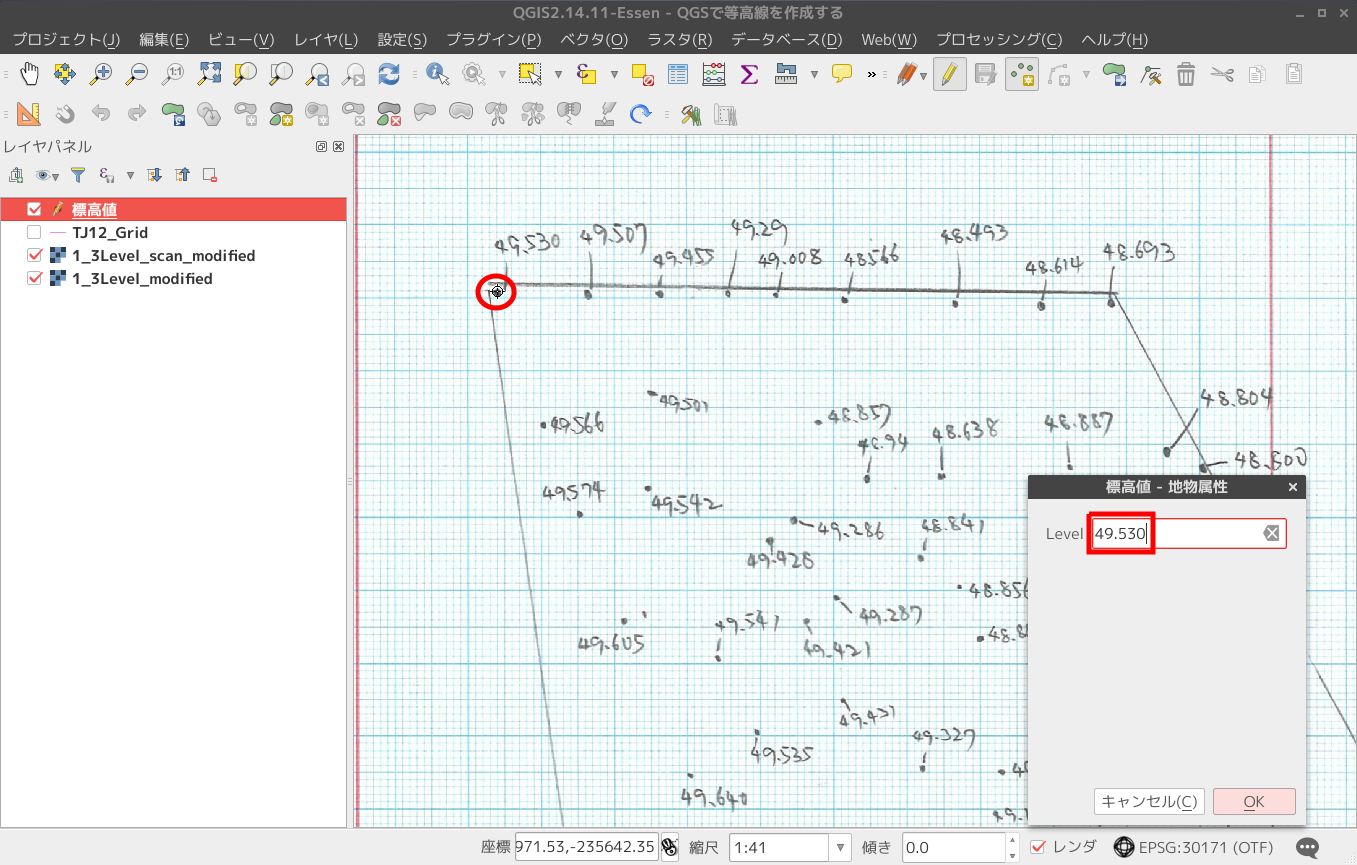
\includegraphics[width=1\linewidth]{08.png}
\caption{幾何補正した紙図面から標高データを取得}
\end{figurehere}

%%%%
\section{標高ラスタを作成する}
「空間補完(ラスタ内挿)」は標高値のない地点の標高を推定する手法です。生成されるデータはラスタデータです。

\begin{tabular}{l l}
入力ファイル&標高の入ったポイントデータ\\
Zフィールド&標高の入ったフィールド\\
アルゴリズム&「指数逆分布」が一番なめらか\\
指数&2.0〜4.0くらい\\
\end{tabular}

\begin{figurehere}
\centering
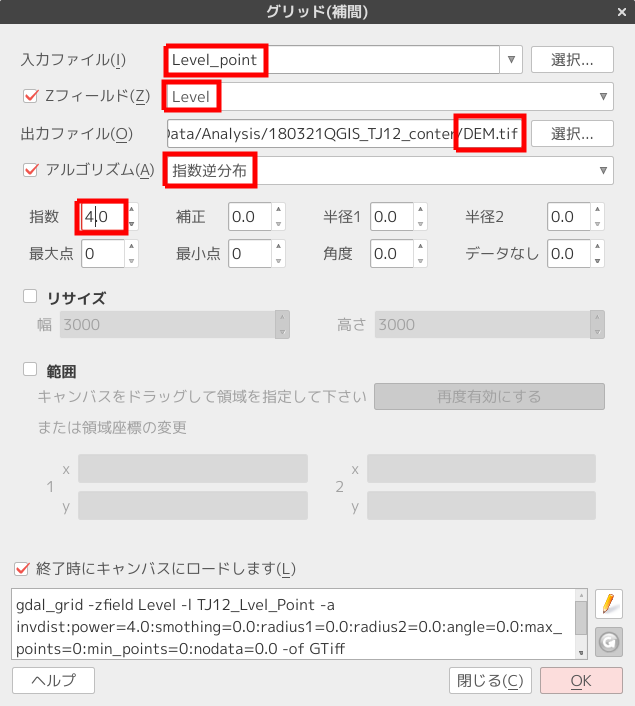
\includegraphics[width=0.8\linewidth]{12.png}
\caption{「グリッド補完」で標高ラスタ作成}
\end{figurehere}

\begin{figurehere}
\centering
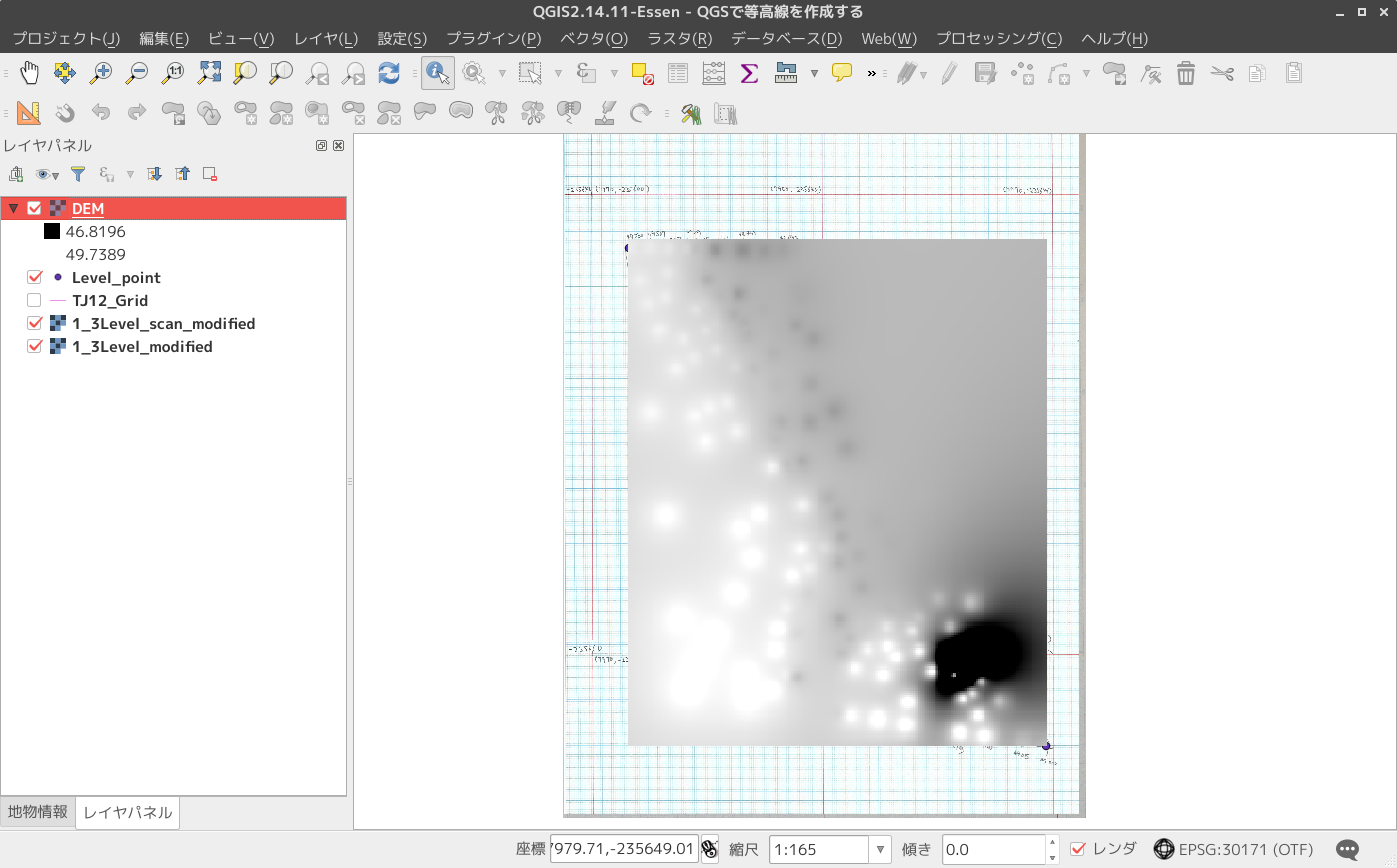
\includegraphics[width=1\linewidth]{13.png}
\caption{作成した標高ラスタ}
\end{figurehere}

%%%%
\section{カラーパレットの選び方}
QGISにはデフォルトで「Color Brewer」によるカラーパレットがインストールされています。QGISにインストールされている「Color Brewer」は連続量を扱うためのパレットが中心です\footnote{
Color Brewerには離散量を扱うための「SET1〜3」や「Accent」なども存在しますが、QGISにはなぜか連続量を扱うカラーパレットしか用意されていません。
}。
離散量(植生図や土地分類図)を扱うためには別のカラーパレットをロードするか、自作してください。

また、マイナス値からプラス値の幅をもつデータとプラス値(或いはマイナス値)のみの幅をもつデータでは選ぶべきカラーパレットが異なります。「Yl-Gr」や「Greens」などはプラス値のみ、「Spectral」などはマイナスからプラスの幅をもつデータに使用するのが適切です。

\begin{figurehere}
\centering
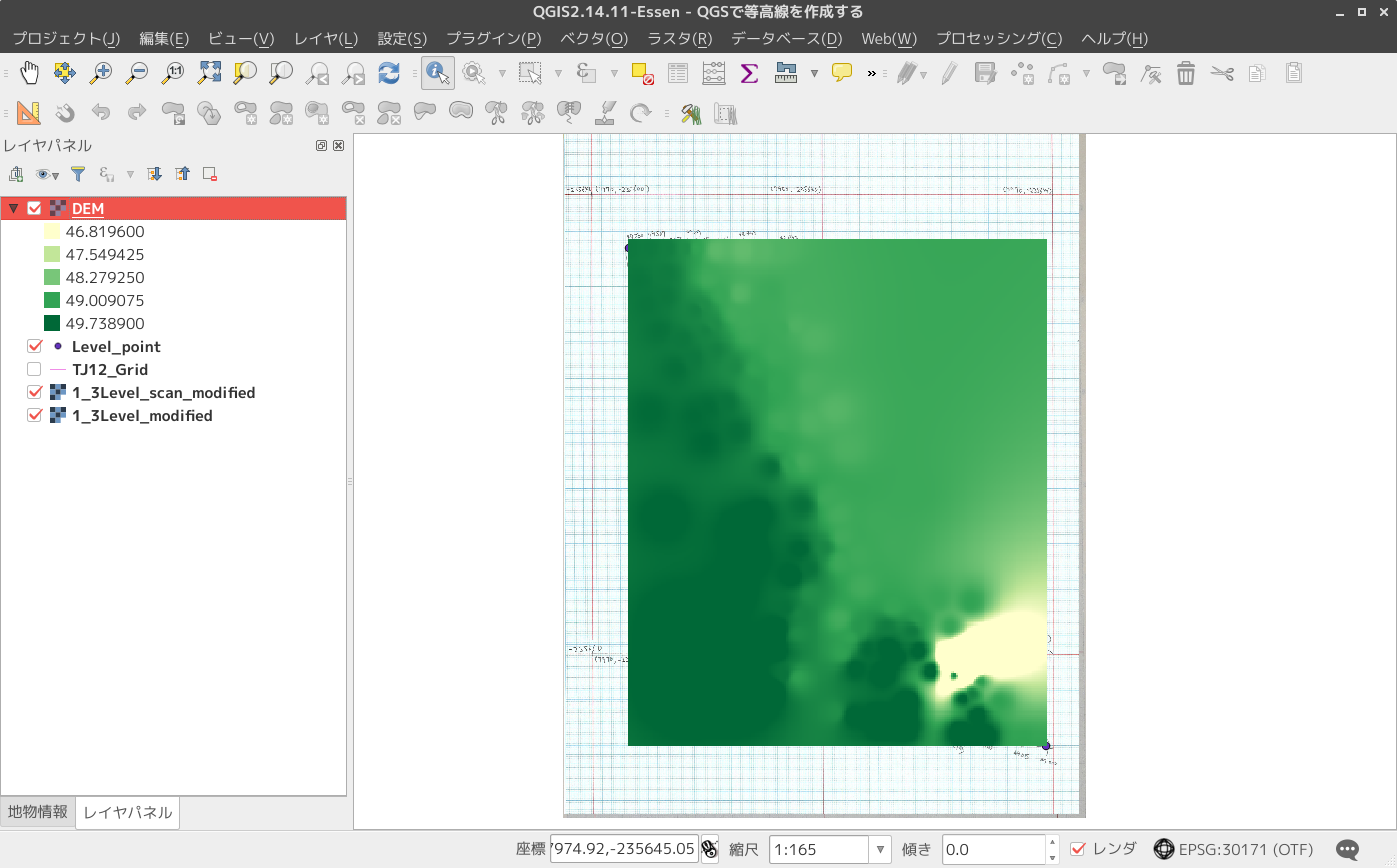
\includegraphics[width=1\linewidth]{14.png}
\caption{「Yl-Gr」による表現}
\end{figurehere}

\begin{figurehere}
\centering
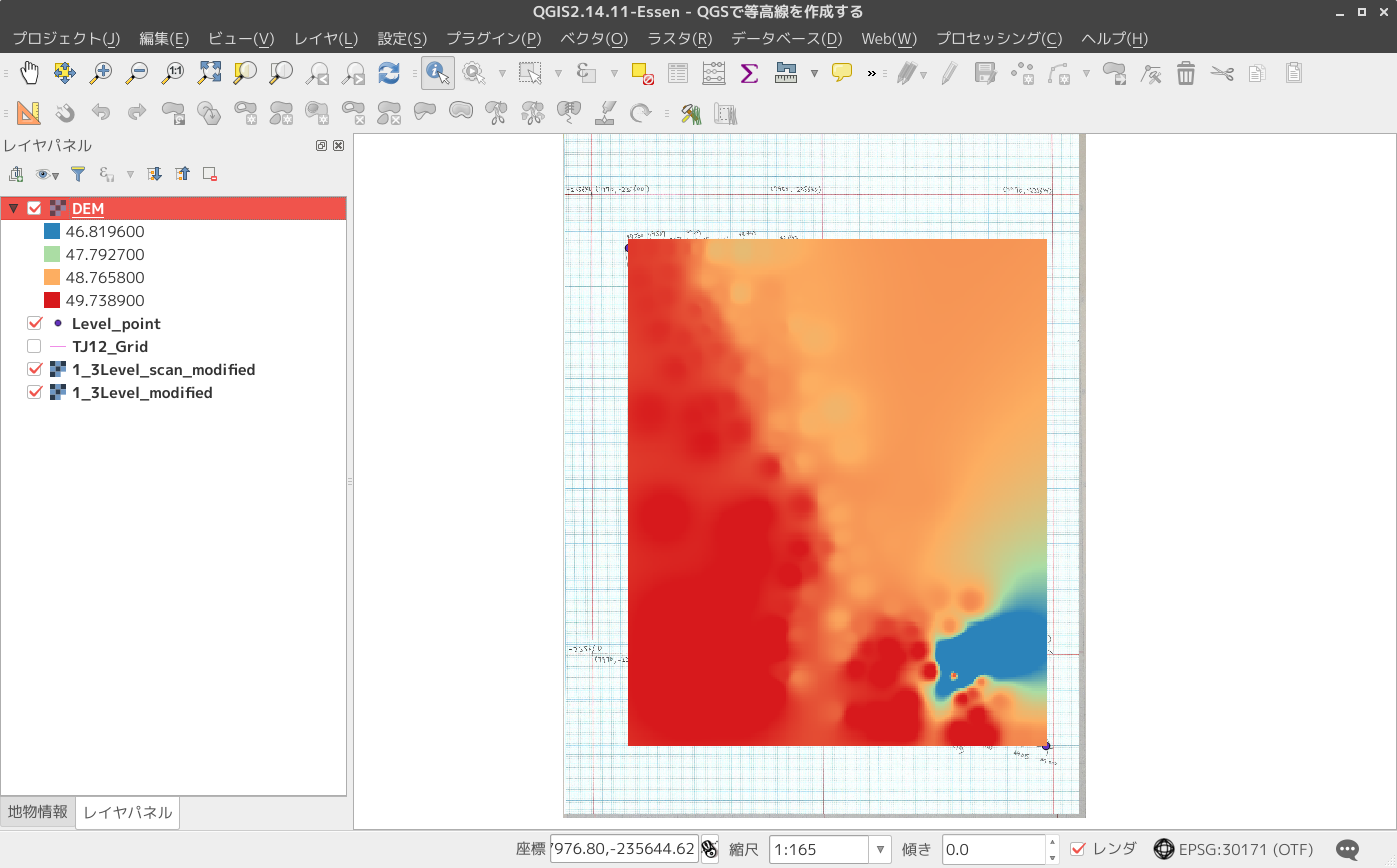
\includegraphics[width=1\linewidth]{15.png}
\caption{「Spectral」による表現}
\end{figurehere}


%%%%
\section{等高線の出力}
ラスタデータから等高線を出力します。単バンドのラスタとして表現されているデータなら何でも等高線が出力できます。遺物の密度ラスタから等密度線を出力することや降雨量ラスタから等雨量線を出力することも同じ手法で実現できます。「傾向面分析」とも呼ばれる解析方法で、傾向面を表現するさまざまな関数が開発されていますが、連続量の分布を調べるためのもっとも基本的な解析方法でもあります。


\begin{tabular}{l l}
入力ファイル&「DEM」\\
等高線間隔&「0.1」\\
ファイル名&「contour」\\
ファイルの種類&「Shapefile」\\
エンコード&「UTF-8」\\
\end{tabular}

\begin{figurehere}
\centering
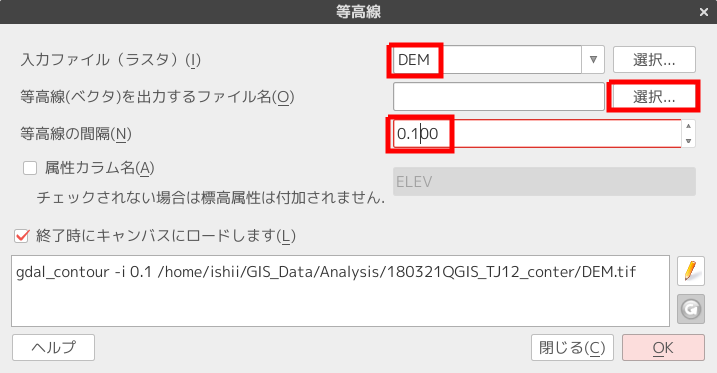
\includegraphics[width=0.8\linewidth]{19.png}
\caption{等高線の作成}
\end{figurehere}


\begin{figurehere}
\centering
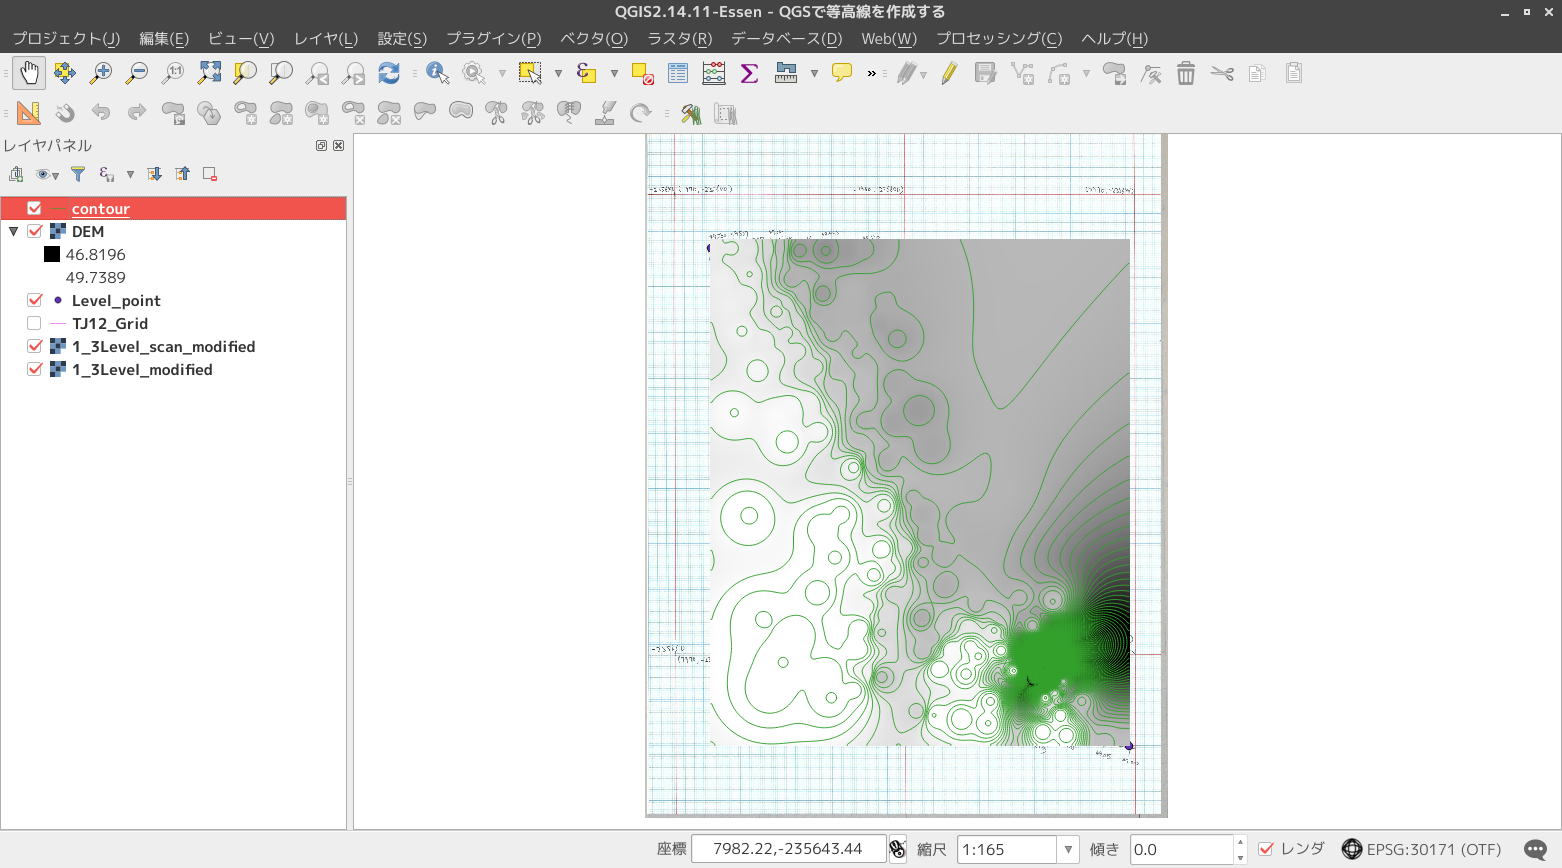
\includegraphics[width=1\linewidth]{21.png}
\caption{標高ラスタから作成された等高線}
\end{figurehere}


%%%%
\section{陰影図を作成}
より視覚的に地形を把握するために陰影図を作成します。

\begin{tabular}{l l}
標高レイヤ&「DEM」\\
出力形式&「GeoTIFF」\\
Zファクタ&「2」\\
\end{tabular}

\begin{figurehere}
\centering
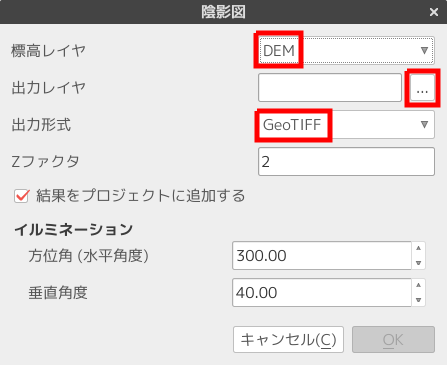
\includegraphics[width=0.6\linewidth]{23.png}
\caption{陰影図作成}
\end{figurehere}

\begin{figurehere}
\centering
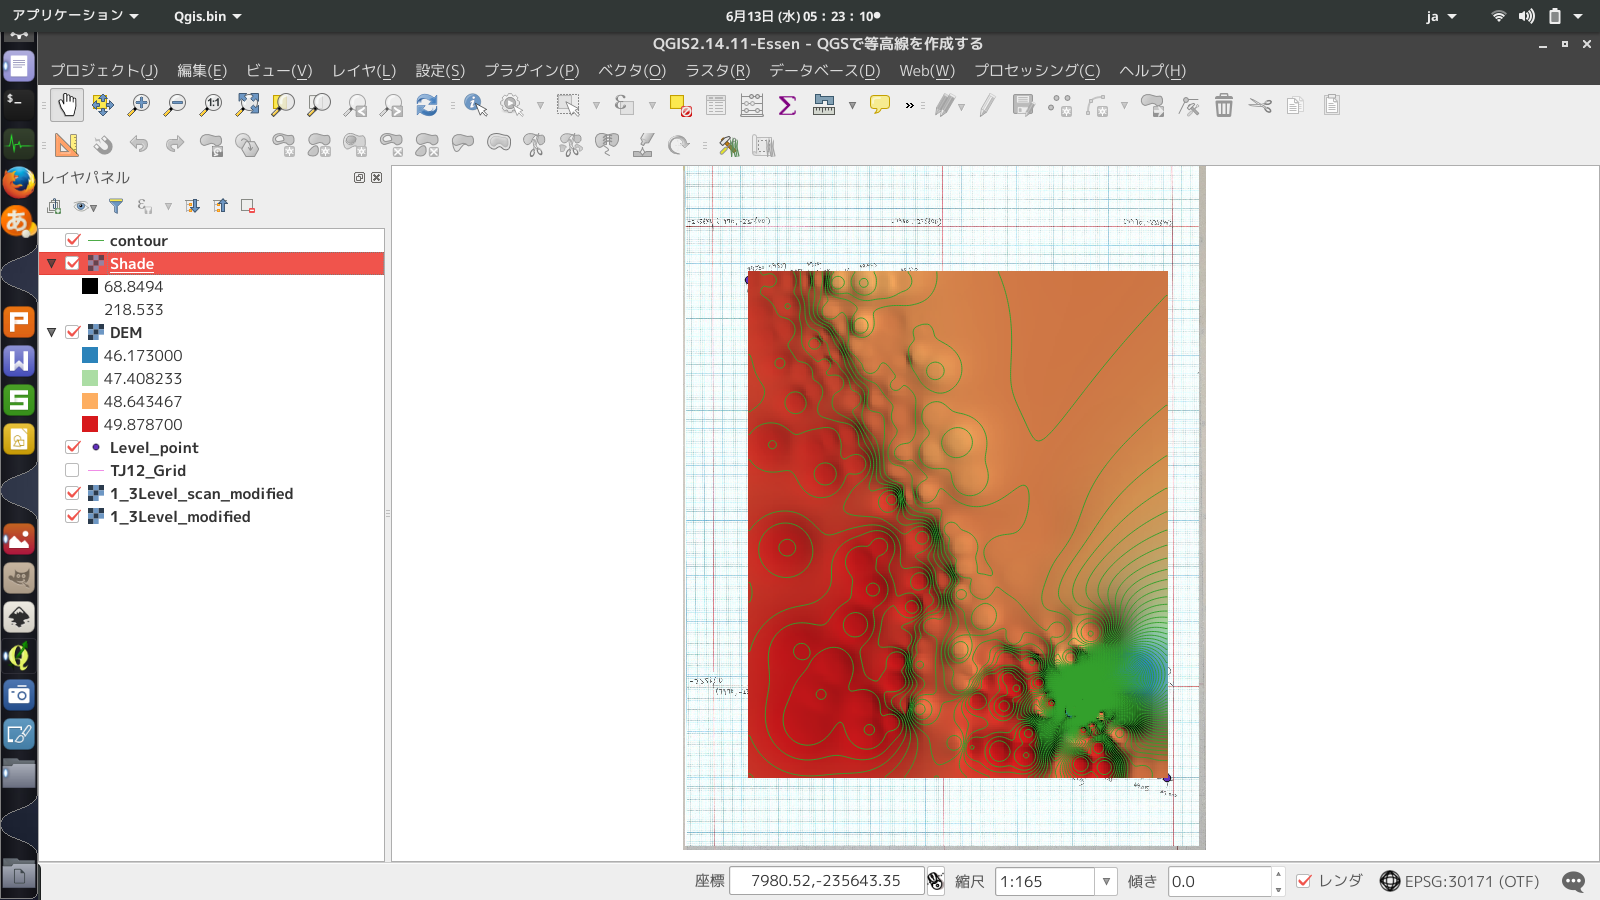
\includegraphics[width=1\linewidth]{28.png}
\caption{「乗算」で重ね合わせた陰影図}
\end{figurehere}


%%%%
\section{調査区ポリゴンの作成}
調査区の形状で他のオブジェクトを切り抜きます。視覚的な意味だけではなく、たとえば河川流域単位で分析を行う場合などに分析に必要な範囲を限定するために必要となります。クリップ(外側の切り抜き)やマスク(内側の切り抜き)では「面」としての性質が必要となります。見た目はよく似ていますが「ライン」を使用するべきなのか、「ポリゴン」を使用するべきなのかはデータの処理によって決まります。

\begin{enumerate}
\item 「新規シェープファイルレイヤ」作成
\item 編集モード切替
\item  ポリゴン地物を追加して調査区をトレース
\end{enumerate}

\begin{figurehere}
\centering
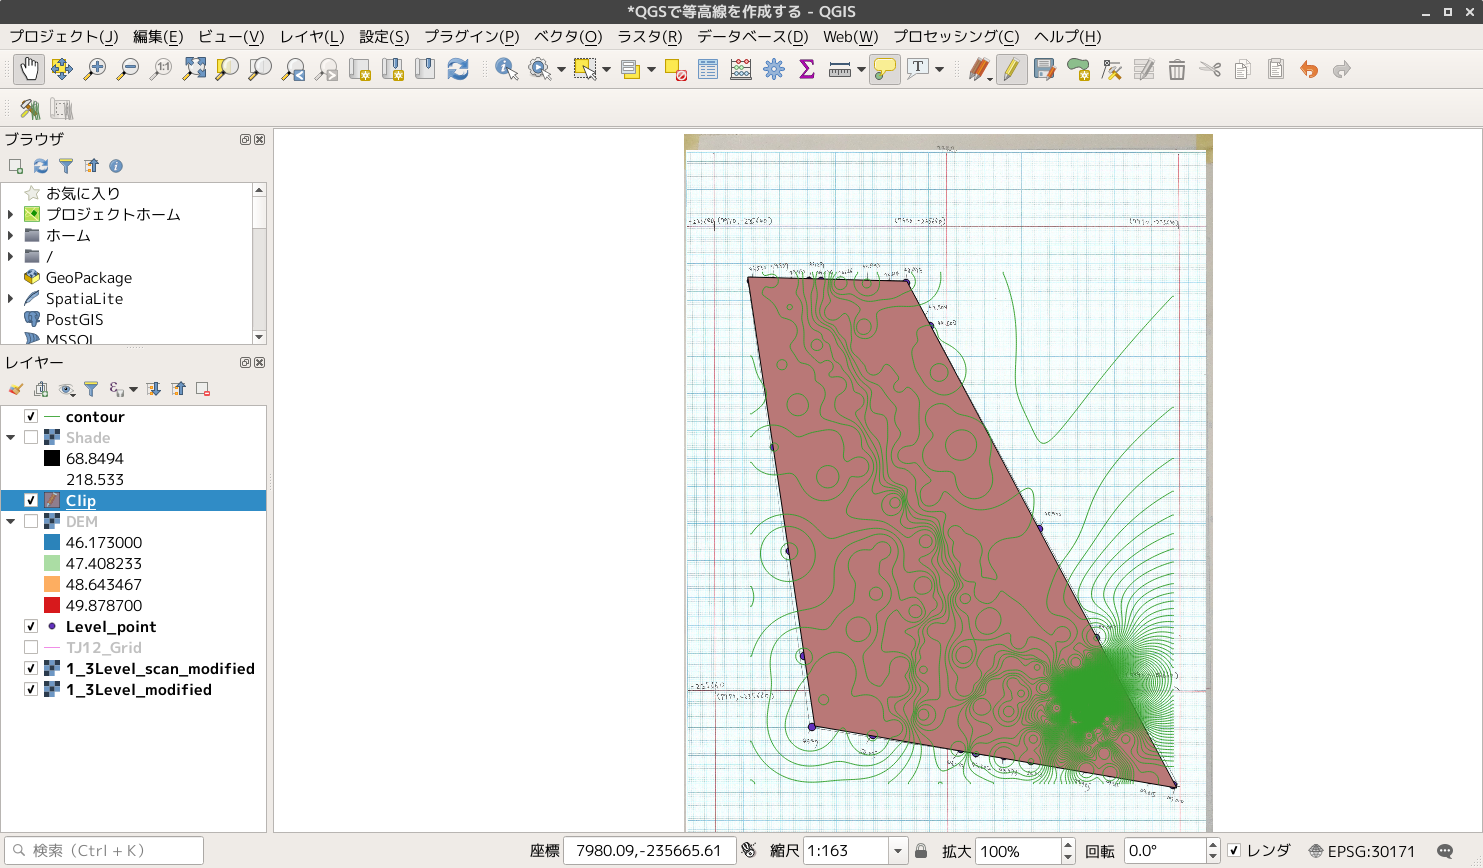
\includegraphics[width=1\linewidth]{36.png}
\caption{調査区のポリゴンデータを作成}
\end{figurehere}

%%%%
\section{調査区ポリゴンで等高線を切り抜く}
ベクタ(調査区ポリゴン)でベクタ(等高線)を切り抜きます。ベクタ同士の幾何学的処理にはクリップのほかにディゾルブ(融合)を使う機会が多いと思います。

「ベクタ」→「空間演算ツール」→「クリップ」
\begin{tabular}{l l}
「入力レイヤ」&クリップされるデータ(等高線)\\
「クリップレイヤ」&クリップする範囲(調査区)\\
\end{tabular}

\begin{figurehere}
\centering
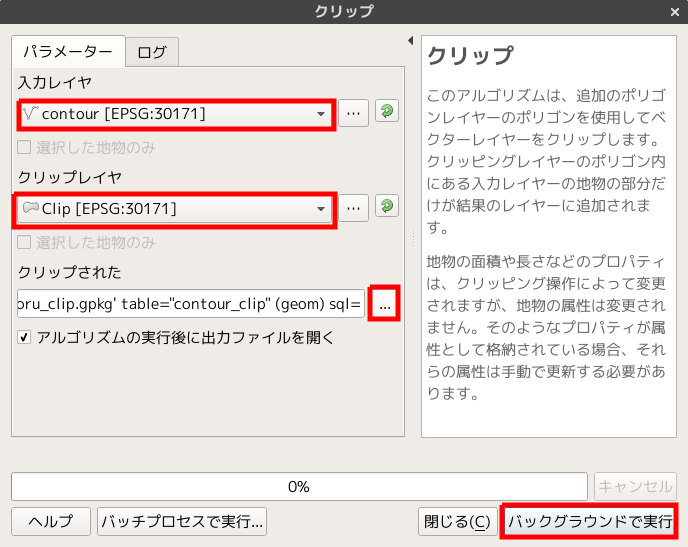
\includegraphics[width=0.8\linewidth]{37.png}
\caption{ベクタデータのクリップ}
\end{figurehere}

\begin{figurehere}
\centering
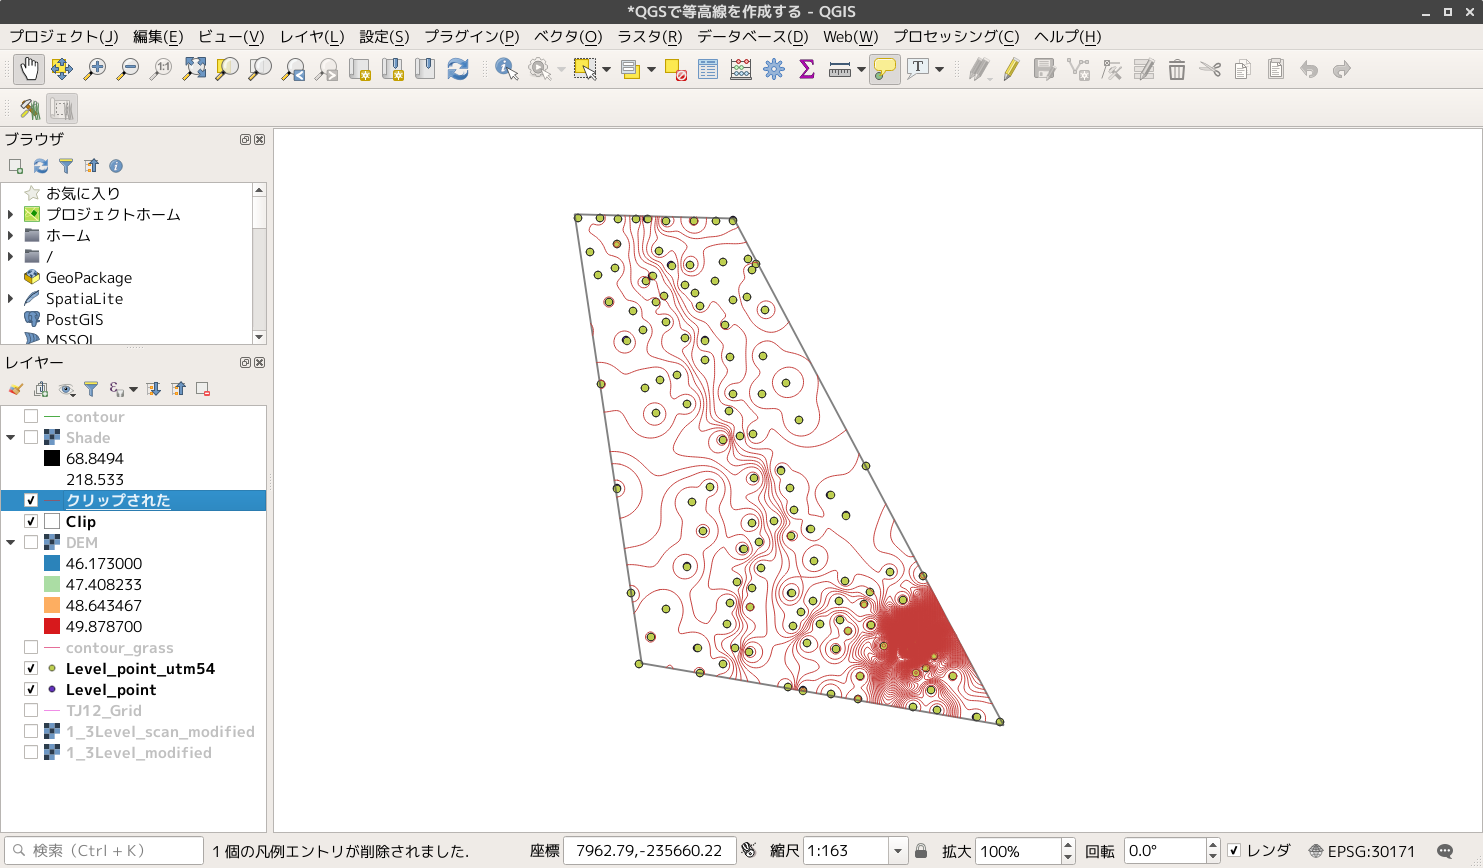
\includegraphics[width=1\linewidth]{39.png}
\caption{調査区で切り抜かれた等高線}
\end{figurehere}

%%%%
\section{調査区ポリゴンでラスタデータを切り抜く}
ベクタでラスタをクリップします。

「ラスタ」→「抽出」→「マスクレイヤによるラスタのクリップ」

\begin{figurehere}
\centering
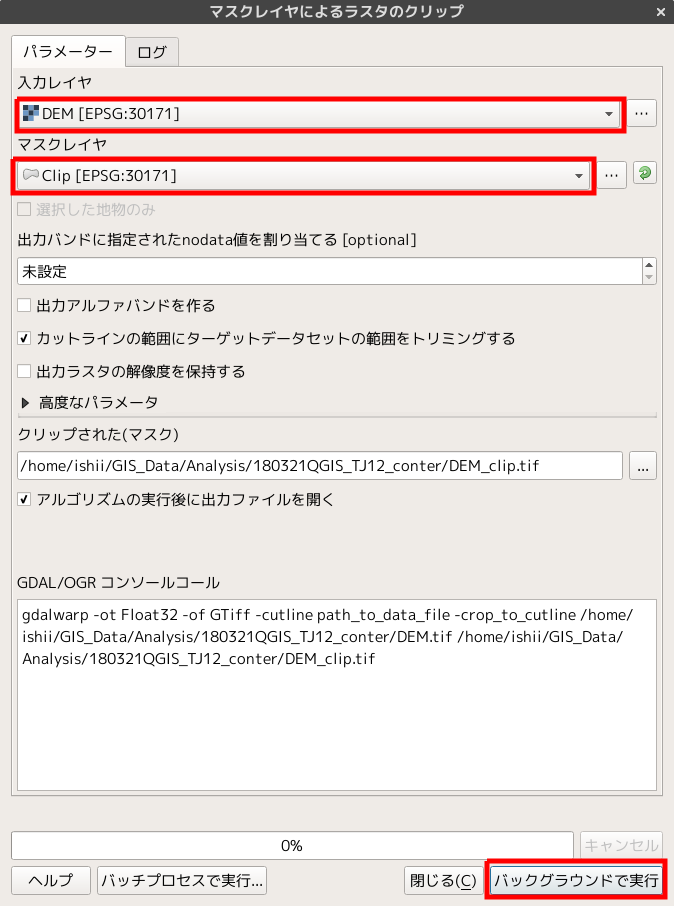
\includegraphics[width=0.5\linewidth]{42.png}
\caption{ラスタデータのクリップ}
\end{figurehere}

\begin{figurehere}
\centering
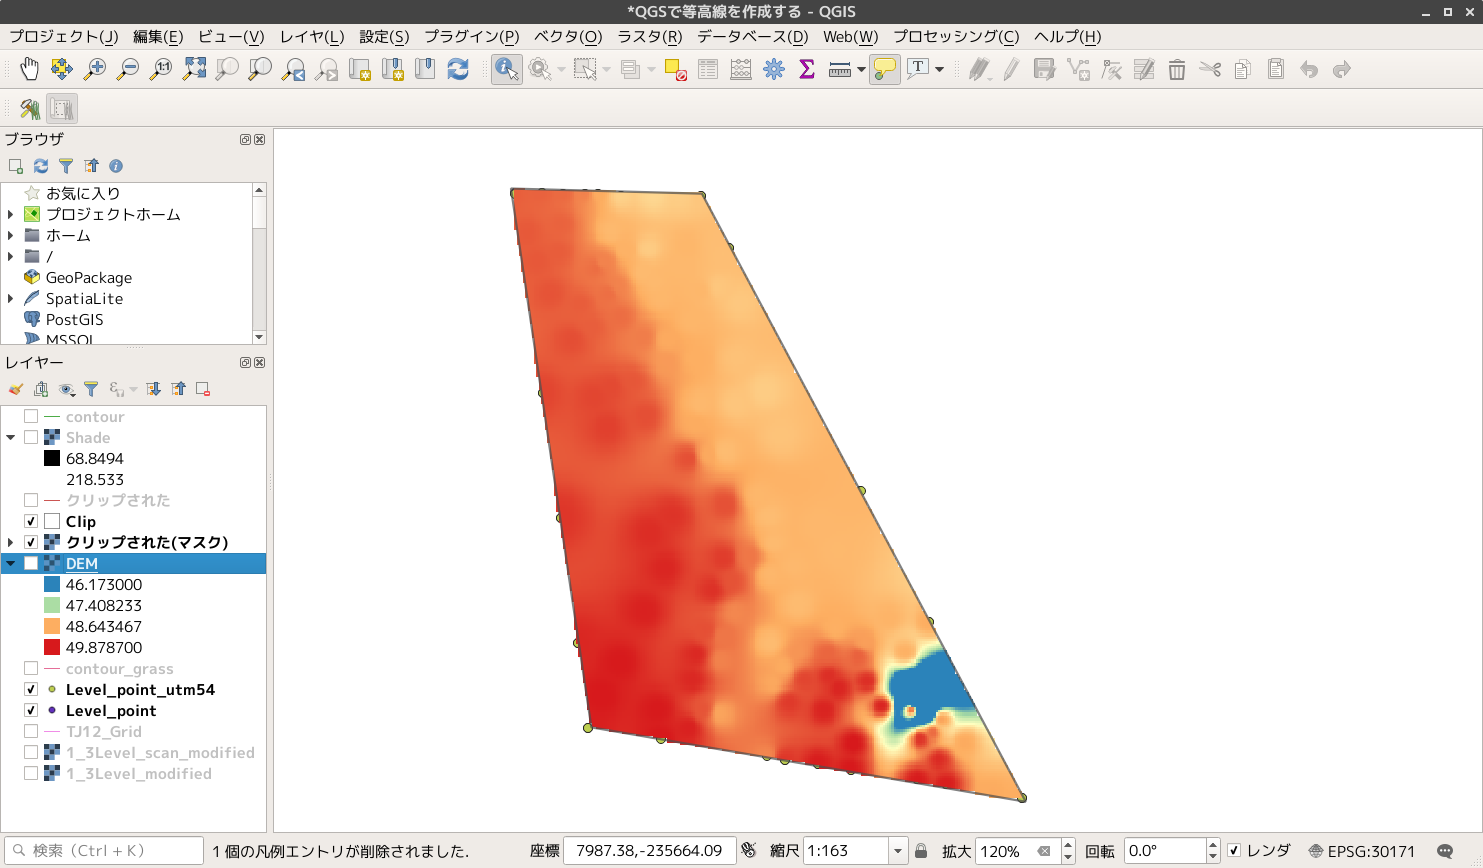
\includegraphics[width=1\linewidth]{43.png}
\caption{クリップされたラスタデータ}
\end{figurehere}

%%%%
\section{滑らかな等高線と測量の密度}
今回の研修で使用したデータは研修用にあえて紙図面を作成しました。実際の整理作業ではトータルステーションを用いて行った測量データをインポートしています。GISで機械的に等高線を生成する場合には、「どの地点の標高を測るべきか」ということが結果に重要な影響を与えます。測量の効率と精度を両立させるためには現場段階でテストを繰り返す必要がありそうです。

\begin{figurehere}
\centering
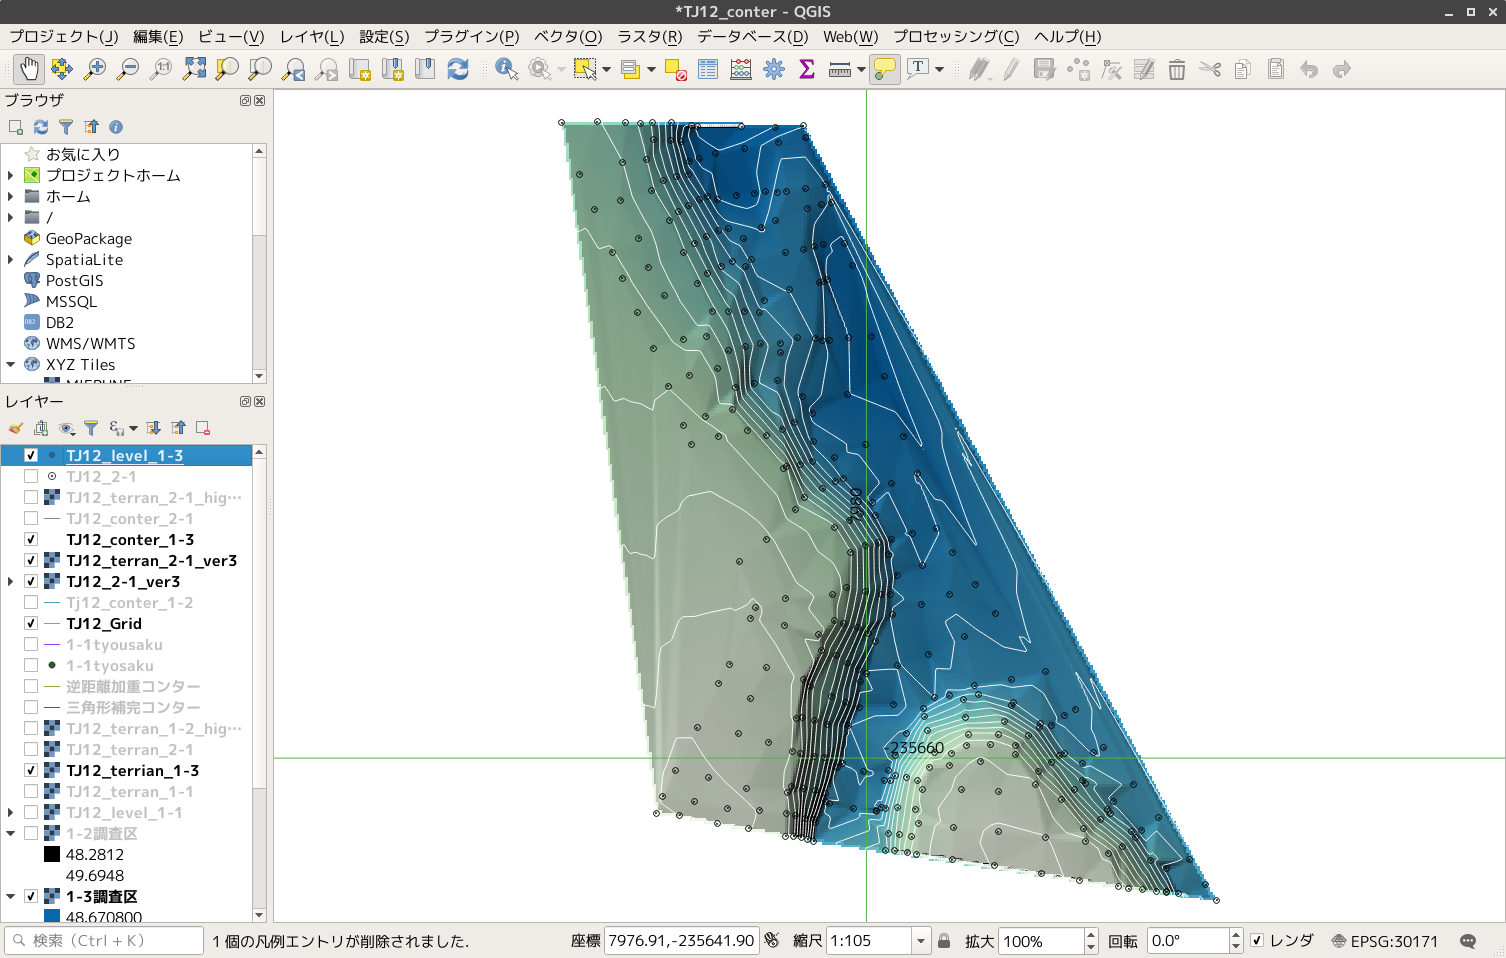
\includegraphics[width=1\linewidth]{44.png}
\caption{実際の整理作業で作成したデータ}
\end{figurehere}


%\end{multicols}
\end{document}
